%%%%%%%%%%%%%%%%%%%%%%%%%%%%%%%%%%%%%%%%%
% Beamer Presentation
% LaTeX Template
% Version 1.0 (10/11/12)
%
% This template has been downloaded from:
% http://www.LaTeXTemplates.com
%
% License:
% CC BY-NC-SA 3.0 (http://creativecommons.org/licenses/by-nc-sa/3.0/)
%
%%%%%%%%%%%%%%%%%%%%%%%%%%%%%%%%%%%%%%%%%

%----------------------------------------------------------------------------------------
%	PACKAGES AND THEMES
%----------------------------------------------------------------------------------------

\documentclass{beamer}

\mode<presentation> {

% The Beamer class comes with a number of default slide themes
% which change the colors and layouts of slides. Below this is a list
% of all the themes, uncomment each in turn to see what they look like.

%\usetheme{default}
%\usetheme{AnnArbor}
%\usetheme{Antibes}
%\usetheme{Bergen}
%\usetheme{Berkeley}
%\usetheme{Berlin}
%\usetheme{Boadilla}
%\usetheme{CambridgeUS}
%\usetheme{Copenhagen}
%\usetheme{Darmstadt}
%\usetheme{Dresden}
%\usetheme{Frankfurt}
%\usetheme{Goettingen}
%\usetheme{Hannover}
%\usetheme{Ilmenau}
%\usetheme{JuanLesPins}
%\usetheme{Luebeck}
%\usetheme{Madrid}
\usetheme{Malmoe}
%\usetheme{Marburg}
%\usetheme{Montpellier}
%\usetheme{PaloAlto}
%\usetheme{Pittsburgh}
%\usetheme{Rochester}
%\usetheme{Singapore}
%\usetheme{Szeged}
%\usetheme{Warsaw}

% As well as themes, the Beamer class has a number of color themes
% for any slide theme. Uncomment each of these in turn to see how it
% changes the colors of your current slide theme.

%\usecolortheme{albatross}
%\usecolortheme{beaver}
%\usecolortheme{beetle}
%\usecolortheme{crane}
%\usecolortheme{dolphin}
%\usecolortheme{dove}
%\usecolortheme{fly}
%\usecolortheme{lily}
%\usecolortheme{orchid}
%\usecolortheme{rose}
%\usecolortheme{seagull}
%\usecolortheme{seahorse}
%\usecolortheme{whale}
%\usecolortheme{wolverine}

%\setbeamertemplate{footline} % To remove the footer line in all slides uncomment this line
%\setbeamertemplate{footline}[page number] % To replace the footer line in all slides with a simple slide count uncomment this line

%\setbeamertemplate{navigation symbols}{} % To remove the navigation symbols from the bottom of all slides uncomment this line
}

\usepackage{graphicx} % Allows including images
\usepackage{booktabs} % Allows the use of \toprule, \midrule and \bottomrule in tables
\usepackage{listings}


% -------------------------------------------
% --- Added by me!
\lstMakeShortInline{!}

\usepackage{tikz}
\usetikzlibrary{positioning,calc}
\tikzset{onslide/.code args={<#1>#2}{%
  \only<#1>{\pgfkeysalso{#2}} % \pgfkeysalso doesn't change the path
}}

\makeatletter
\newenvironment<>{btHighlight}[1][]
{\begin{onlyenv}#2\begingroup\tikzset{bt@Highlight@par/.style={#1}}\begin{lrbox}{\@tempboxa}}
{\end{lrbox}\bt@HL@box[bt@Highlight@par]{\@tempboxa}\endgroup\end{onlyenv}}

\newcommand<>\btHL[1][]{%
  \only#2{\begin{btHighlight}[#1]\bgroup\aftergroup\bt@HL@endenv}%
}
\def\bt@HL@endenv{%
  \end{btHighlight}%   
  \egroup
}
\newcommand{\bt@HL@box}[2][]{%
  \tikz[#1]{%
    \pgfpathrectangle{\pgfpoint{1pt}{0pt}}{\pgfpoint{\wd #2}{\ht #2}}%
    \pgfusepath{use as bounding box}%
    \node[anchor=base west, fill=orange!30,outer sep=0pt,inner xsep=1pt, inner ysep=0pt, rounded corners=3pt, minimum height=\ht\strutbox+1pt,#1]{\raisebox{1pt}{\strut}\strut\usebox{#2}};
  }%
}
\makeatother

\usepackage{caption}
\captionsetup{font=scriptsize,labelfont=scriptsize,justification=centering}

% -----------------------------------------------------

%----------------------------------------------------------------------------------------
%	TITLE PAGE
%----------------------------------------------------------------------------------------

\title[Host Compiled Simulation]{Host Compiled Simulation\\for Timing and Power Estimation} % The short title appears at the bottom of every slide, the full title is only on the title page

\author{Gaurav Kukreja} % Your name
\institute[TUM] % Your institution as it will appear on the bottom of every slide, may be shorthand to save space
{
Technical University of Munich\\ % Your institution for the title page
\medskip
\textit{gaurav@gauravk.in} % Your email address
}
\date{\today} % Date, can be changed to a custom date

\begin{document}

\definecolor{codegray}{rgb}{0.5,0.5,0.5}
\definecolor{mygreen}{rgb}{0,0.8,0.6}
\definecolor{myorange}{rgb}{1.0,0.4,0}

\lstset{frame=single,
  language=C++,
  aboveskip=3mm,
  belowskip=3mm,
  showstringspaces=false,
  basicstyle={\fontsize{7}{9}\selectfont\ttfamily},
  commentstyle={\itshape\color{codegray}},
  numberstyle={\fontsize{4}{6}\selectfont\ttfamily\color{codegray}},
  keywordstyle=\color{mygreen},
  stringstyle=\color{myorange},
  columns=flexible,
  numbers=left,
  xleftmargin=3em,
  framexleftmargin=2em,
  breaklines=true,
  breakatwhitespace=true,
  tabsize=4,
  captionpos=b,
  moredelim={**[is][\btHL<1>]{@1}{@}},
  moredelim={**[is][\btHL<2>]{@2}{@}}
}

\begin{frame}
\titlepage % Print the title page as the first slide
\end{frame}

\begin{frame}
\frametitle{Overview} % Table of contents slide, comment this block out to remove it
\tableofcontents[
  currentsection,
  sectionstyle=show,
  subsectionstyle=hide
]
\end{frame}

%----------------------------------------------------------------------------------------
%	PRESENTATION SLIDES
%----------------------------------------------------------------------------------------

%------------------------------------------------
\section{Introduction} 
%------------------------------------------------

\subsection{Simulation}
\begin{frame}
\frametitle{Simulation}
Simulation is the technique to imitate the behaviour of a system.
\begin{itemize}
\item Widely used in Hardware Software Co-development.
\item Use cases are performance analysis, functional verification etc.
\end{itemize}
\end{frame}

\begin{frame}
\frametitle{Simulation: Popular Techniques}
\textbf{Instruction Set Simulation}
\begin{itemize}
\item Detailed simulation of processor micro-architecture.
\item Cycle Accurate estimation of performance.
\item Difficult to develop, Very Slow execution.
\end{itemize}
\textbf{Functional Simulation}
\begin{itemize}
\item Simulation at higher level of abstraction. Details of micro-architecture ignored. 
\item Very fast simulation.
\item Focus is Functional Verification. Cannot be used for performance estimation.
\end{itemize}
\end{frame}

\subsection{Focus}
\begin{frame}
\frametitle{Our Focus}
A technique for fast simulation of embedded processors that is,
\begin{itemize}
\item Easy to Develop.
\item Fast to Execute.
\item Highly Accurate in Performance Estimation.
\end{itemize}
\end{frame}

%\subsection{Related Work}
%\begin{frame}
%\frametitle{Related Work}
%\textbf{Sampling Based Approach}
%\begin{itemize}
%\item Instead of executing entire application using ISS, certain samples from the execution trace are selected which are simulated in detail using ISS. Rest of the simulation is done using FS.
%\item Results from detailed simulation are interpolated to estimate performance.
%\item Accuracy highly dependent on how samples are chosen.
%\item Difficult to develop ISS.
%\end{itemize}
%\end{frame}

\subsection{Host Compiled Simulation}
\begin{frame}
\frametitle{Host Compiled Simulation}
\textbf{Host Compiled Simulation}
\begin{itemize}
\item Based on technique of Source Code Instrumentation.
\item Instrumented code run on Host Machine, hence the name.
\item Easy to understand, develop and maintain.
\item Fast Execution, and accurate results.
\end{itemize}
\end{frame}

\begin{frame}[fragile]
\frametitle{Simple Example}
%\textbf{Short Example}
%\begin{columns}
\begin{minipage}{.5\textwidth}
\begin{lstlisting}[caption={Simple C Code},label={lst:sumCCode}]
int sum(int array[20])
{
    int i;
    int sum = 0;
	
    for (i=0; i<20; i++)
        sum += array[i];
	
    return sum;
}
\end{lstlisting}
\end{minipage}%
\begin{minipage}{.5\textwidth}
\begin{lstlisting}[caption={Objdump Code},label={lst:sumObjCode}]
00008068 <sum>:
8068:     mov     r3, #0
806c:     mov     r2, r3
8070:     ldr     r1, [r0, r3]
8074:     add     r2, r2, r1
8078:     add     r3, r3, #4
807c:     cmp     r3, #80 ; 0x50
8080:     bne     8070 <sum+0x8>
8084:     mov     r0, r2
8088:     bx      lr
\end{lstlisting}
\end{minipage}

\begin{table}[b]
\fontsize{8}{10}\selectfont
\begin{center}
\begin{tabular}{cccc}
\toprule
	\multicolumn{2}{c}{Basic Block in Binary} & \multicolumn{2}{c}{Matching block in Source}\\ 
	\midrule
	BlockID & Lines & BlockID & Lines \\
    \hline
	1 & 2-3 & 1 & 3-4 \\
	2 & 4-8 & 2 & 7 \\
	3 & 9-10 & 3 & 9 \\	
\bottomrule
\end{tabular}
%\caption{Mapping of Basic Blocks}
\end{center}
\end{table}
\end{frame}

\begin{frame}[fragile]
\frametitle{Instrumented Code}
\begin{minipage}{.62\textwidth}
\begin{lstlisting}[caption={Instrumented Code},label={lst:sumInstCode},
                    basicstyle={\fontsize{6}{8}\selectfont\ttfamily}]
@1unsigned int execCycles;@
@1unsigned int memAccessCycles;@

int sum(int array[20])
{
    int i;
    int sum = 0;
    @1execCycles += 2;@
    @1memAccessCycles += simICache(0x8068, 8);@
	
    for (i=0; i<20; i++)
    {
        sum += array[i];
        @1memAccessCycles += simDCache(&array + i, READ);@
        @1execCycles += 5;@
        @1memAccessCycles += simICache(0x8070, 40);@
    }
	
    @1execCycles += 2;@
    @1memAccessCycles += simICache(0x8084, 8);@
    return sum;
}
\end{lstlisting}
\end{minipage}%
\begin{minipage}{0.38\textwidth}
\begin{lstlisting}[basicstyle={\fontsize{6}{8}\selectfont\ttfamily},aboveskip=0mm,belowskip=2mm]
int sum(int array[20])
{
    int i;
    int sum = 0;
	
    for (i=0; i<20; i++)
        sum += array[i];
	
    return sum;
}
\end{lstlisting}
\begin{lstlisting}[basicstyle={\fontsize{6}{8}\selectfont\ttfamily},aboveskip=2mm,belowskip=5mm]
00008068 <sum>:
8068:     mov     r3, #0
806c:     mov     r2, r3
8070:     ldr     r1, [r0, r3]
8074:     add     r2, r2, r1
8078:     add     r3, r3, #4
807c:     cmp     r3, #80 ; 0x50
8080:     bne     8070 <sum+0x8>
8084:     mov     r0, r2
8088:     bx      lr
\end{lstlisting}
\end{minipage}
\end{frame}

%\begin{frame}
%\frametitle{Contribution}
%\begin{itemize}
%\item Algorithm for Mapping between Source and Binary Code.
%\item Detailed Cache Simulation for better accuracy.
%\item Accurate Simulation of Processor Pipeline.
%\item Using Power State Model for Power Estimation.
%\end{itemize}
%\end{frame}

\begin{frame}
\frametitle{Objective}
\begin{itemize}
\item Develop a tool for Automatic Instrumentation.
\item ARM Cortex A5 based processor as reference target device.
\item Bare-Metal Applications.
\item Generate Time and Power Consumption Estimates.
\end{itemize}
\end{frame}

%------------------------------------------------

\section{Timing Estimation}

\subsection{Outline}

\begin{frame}
\frametitle{Outline of our Approach}
\begin{itemize}
\item Generate Mapping between Source Code and Binary Code.
\item Extract Information from GDB
\item Data Cache Simulation
\item Instruction Cache Simulation
\item Annotation for cycles spent in Pipeline
\end{itemize}
\end{frame}

\subsection{Mapping between Source and Binary}

\begin{frame}
\frametitle{Mapping between Source and Binary}
\begin{itemize}
\item Accurate mapping is needed for instrumentation.
\item Compiler destroys mapping during optimization phases.
\item GDB provides mapping, but highly inaccurate.
\item Algorithms use static and dynamic analysis of Control and Data Flow.
\end{itemize}
\end{frame}

\begin{frame}
\frametitle{Mapping between Source and Binary}
In this project, mapping is generated using following steps.
\begin{itemize}
\item Cross-Compile Source Code.
\item Convert IR Code to C Code (Intermediate Source Code).
\item Extract CFG from ISC and Binary Code.
\item Map CFGs using Matching Algorithm
\end{itemize}
\end{frame}

\begin{frame}
\frametitle{Conversion of IR Code to C Code}
\begin{itemize}
\item IR Code already contains front-end (processor independent) optimizations. Control Flow closer to Binary Code.
\item IR Code is in GIMPLE format. 
\item GIMPLE Code is converted to C Code.
\item The generated code is called Intermediate Source Code (ISC).
\end{itemize}
\end{frame}

\begin{frame}
\frametitle{Mapping Algorithm}
\begin{itemize}
\item ISC and object dump of binary code is parsed, and CFGs are extracted.
\item Graphs are traversed recursively in Depth First Fashion, to match each branch.
\item Special Handling for optimizations that modify Control Flow.
\item GDB Debug information in Corner Cases.
\end{itemize}
\end{frame}

\begin{frame}
\begin{minipage}{.5\textwidth}
\begin{figure}
\includegraphics[width=.5\textwidth]{figures/obj_my_ctop_IR_adpcm_coder-crop}
\end{figure}
\end{minipage}%
\begin{minipage}{.5\textwidth}
\begin{figure}
\includegraphics[height=.9\textheight]{figures/isc_adpcm_IR_adpcm_coder-crop}
\end{figure}
\end{minipage}
\end{frame}

\subsection{Data Cache Simulation}

\begin{frame}
\frametitle{Data Cache Simulation}
\begin{itemize}
\item For accurately annotating time spent in memory access, data cache must be simulated.
\item Cache Simulator to imitate the cache on Target Processor is needed.
\item Host Addresses can not be used for Cache Simulation. (???)
\item Memory access, as it would occur on the target processor, needs to be simulated.
\end{itemize}
\end{frame}

\begin{frame}
\frametitle{Cache Simulator}
The device used for testing uses ARM Cortex A5. The cache hierarchy used in target processor has been implemented in the Cache Simulator
\begin{table}
\centering
\begin{tabular}{c|ccc}
        &  Size   & N-way   & Cache Line Size \\
    \hline
    L1 D Cache  & 32 KB & 4 & 32 B \\
    L1 I Cache  & 32 KB & 2 & 32 B \\
    L2 Cache    & 256 KB & 16 & 32 B \\
\end{tabular}
\end{table}
\begin{itemize}
\item Pseudo Random Replacement Policy
\item Data Prefetching
\end{itemize}
\end{frame}

\begin{frame}[fragile]
\frametitle{Cache Simulator}
The Cache simulator offers following API for Data Cache Simulation
\begin{lstlisting}[frame=none,numbers=none,basicstyle={\fontsize{9}{11}\selectfont\ttfamily}]
/**
 * @brief Function to simulate Data Cache Access.
 *
 * @param Address of the memory being accessed.
 * @param True, if access is Read Access. 
 *         False, if write access.
 *
 * @return Number of cycles spent in performing access.
 */
unsigned long long simDCache(unsigned long address,
                                unsigned int isReadAccess);
\end{lstlisting}
\end{frame}

\begin{frame}
\frametitle{Memory Access Reconstruction}
For simulation of cache, addresses from Host Machine can not be used. It may lead to inaccuracies because of,
\begin{itemize}
\item Memory Alignment differences.
\item Different Sizes of Basic Data Types
\end{itemize}
Let us look at how to reconstruct each memory access, as it would occur on the target processor.
\end{frame}

\begin{frame}
\frametitle{Memory Access Reconstruction}
\begin{itemize}
\item GDB is used to extract information about each variable used.
\item Binary Code is parsed to identify load/store instructions. 
\item Variable being accessed by the instruction is identified.
\item Each Load/Store instruction is matched to an instruction in Source Code that causes the memory access.
\item Memory access of the variable is appropriately instrumented.
\end{itemize}
\end{frame}

\begin{frame}
\frametitle{Extracting information using GDB}
\begin{itemize}
\item The source code is compiled to run on bare-metal.
\item Physical address of each Global Variable can be extracted statically from the binary using GDB.
\item Address of local variables, relative to the stack pointer can be extracted using GDB.
\end{itemize}
This information will later be used.
\end{frame}

\begin{frame}
\frametitle{Identify Load/Store Operations in Binary Code}
To identify which variable is being accessed by a load/store instruction,
\begin{itemize}
\item The binary code is partially simulated. 
\item Register State is maintained. Each instruction in binary code is parsed, and registers are updated according to the instruction.
\item Branch instructions are ignored, so each instruction is only simulated once.
\item For each load/store instruction, the address being accessed can be known.
\item Using this address and the information extracted from GDB, the variable being accessed can be identified.
\end{itemize}
\end{frame}

\begin{frame}[fragile]
\frametitle{Variables to accumulate statistics}
To accumulate the number of cycles spent in execution of the program, teo global variables are declared.
\begin{itemize}
\item \texttt{execCycles} is used for cycles spent in active state of processor. ie. when instructions are being executed in the pipeline.
\item \texttt{memAccessCycles} is used for cycles spent in fetching data from memory, when the processor is in idle state and pipeline has been stalled.
\end{itemize}
\begin{lstlisting}[frame=none,numbers=none]
@1unsigned long long execCycles;@
@1unsigned long long memAccessCycles;@
\end{lstlisting}
\end{frame}

\begin{frame}[fragile]
\frametitle{Stack Pointer Simulation}
\begin{itemize}
\item Global Variable \texttt{CSIM\_SP} is declared to maintain the value of Stack Pointer.
\item \texttt{CSIM\_SP} is incremented at the beginning of each function, by the size of the stack frame of the function.
\item Size of stack frame for each function can be known from GDB.
\end{itemize}
\begin{lstlisting}[frame=none,numbers=none]
@1unsigned long CSIM_SP = 0x60c0;@
...
void foo() {
    @1CSIM_SP += 0x30;@
    ...
}
\end{lstlisting}
\end{frame}

\begin{frame}[fragile]
\frametitle{Address of variables on Target}
\begin{itemize}
\item For each Global Variable being used, a new global variable is declared to store the address of the variable in the target processor.
\end{itemize}
\begin{lstlisting}[frame=none,numbers=none]
int array[10];
@1unsigned long array_addr = 0x7c08;@
\end{lstlisting}
\begin{itemize}
\item Similarly, for each local variable a new local variable is declared to store the address of the variable relative to the stack pointer.
\end{itemize}
\begin{lstlisting}[frame=none,numbers=none]
void foo() {
    int average;
    @1unsigned long average_addr = 0x8;@
}
\end{lstlisting}
\end{frame}

\begin{frame}[fragile]
\frametitle{Annotation of Memory Access}
To find the line in source code, which causes the memory access operation,
\begin{itemize}
\item Each line in ISC is parsed using a C parser.
\item The line which causes the load/store operation is identified.
\item The variable being accessed may be an array, indexed by a value. This is identified.
\item Annotation to perform cache simulation is appropriately added.
\item Example ...
\end{itemize}
\end{frame}

\begin{frame}[fragile]
\frametitle{Example: Annotation of Memory Access}
\begin{lstlisting}[frame=none,numbers=none]
...
for (i=0; i<10; i++) {
    sum += array[i];
    @1memAccessCycles += simDCache{array_addr + i * 4, True);@
}
...
average = sum / 10;
@1memAccessCycles += simDCache(SP + average_addr, False);@
...
\end{lstlisting}
\end{frame}

\subsection{Instruction Cache Simulation}

\begin{frame}[fragile]
\frametitle{Cache Simulator}
The Cache simulator offers following API for Instruction Cache Simulation
\begin{lstlisting}[frame=none,numbers=none,basicstyle={\fontsize{9}{11}\selectfont\ttfamily}]
/**
 * @brief Function to simulate Instruction Cache Access.
 *
 * @param Start Address of the basic block.
 * @param Size of the basic block in Bytes.
 *
 * @return Number of cycles spent in performing access.
 */
unsigned long long simICache(unsigned long address,
                                unsigned long size);
\end{lstlisting}
\end{frame}

\begin{frame}
\frametitle{Instruction Cache Simulation}
Annotation for Instruction Cache Simulation is much simpler.
\begin{itemize}
\item For each basic block in binary code, size of the basic block in size is calculated. Start address of the basic block is known.
\item Annotation is added in the beginning of the mapped basic block in the Source Code.
\end{itemize}
\end{frame}

\subsection{Annotation for Cycles spent in Pipeline}

\begin{frame}
\frametitle{Annotation for Cycles spent in Pipeline}
For estimating the cycles spent in pipeline execution, following points need to be considered.
\begin{itemize}
\item Pipeline Architecture of the target processor.
\item Effects due to Data and Control Hazards, that leads to pipeline stalls.
\item Branch Prediction, that prevents pipeline flushes.
\end{itemize}
\end{frame}

\begin{frame}
\frametitle{Pipeline architecture of ARM Cortex A5}
The ARM Cortex A5 has an 8-stage pipeline. The stages are graphically represented below.
\begin{figure}
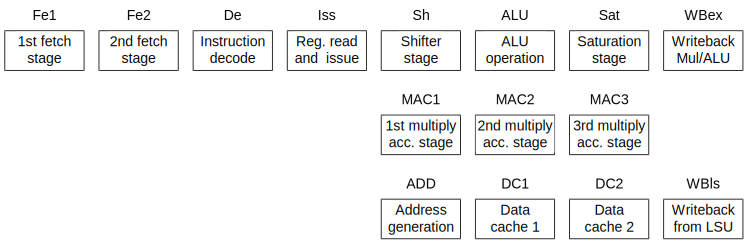
\includegraphics[width=\textwidth]{figures/pipeline}
\end{figure}
\end{frame}

%\begin{frame}
%\frametitle{Effects due to Data and Control Hazards}
%Instructions are executed in a sequence in the processor pipeline. An instruction may need to use data produced by the previous instruction. The result may not be available yet, and the pipeline may need to stall to wait for the data. This situation is called \textbf{Data Hazard}.
%
%Execution Units are used in a processor, which perform instructions like addition, multiplication. Some instructions may need more than one cycle to complete. During this time, the execution unit is reserved. A subsequent instruction may have to wait to use the same execution unit. This is known as \textbf{Control Hazard}.
%
%Compilers try to optimize code by eliminating Data and Control Hazards, but not all can be eliminated.
%\end{frame}

\begin{frame}
\frametitle{Effects due to Data and Control Hazards}
To estimate the number of cycles a basic block will take to execute, 
\begin{itemize}
\item It is assumed, that all data is needed by instructions is available in registers. 
\item Each instruction in the Basic Block is parsed.
\item Initially the pipeline is assumed to be empty.
\item Without interlocking each instruction takes 1 cycle to execute.
\item Interlocking between instructions is identified, and penalties are added.
\end{itemize}
\end{frame}

\begin{frame}[fragile]
\frametitle{Annotation of Cycles spent in Pipeline}
\begin{itemize}
\item For each basic block in Binary code, annotation is added to the mapped Basic Block in the Source Code.
\item The global variable \texttt{execCycles} is incremened by the number of cycles.
\end{itemize}
\begin{lstlisting}[frame=none,numbers=none]
...
for(i<0; i<10; i++) {}
    @1execCycles += 23;@
    sum += array[i];
    ...
}
...
\end{lstlisting}
\end{frame}
%
%\begin{frame}
%\frametitle{Effects due to conditional branching}
%Conditional Branching instructions are used to change the flow of execution, depending on the result of a previous compare instruction.
%\\
%When a conditional branch instruction is fetched into the pipeline, the result of the compare instruction may not be available. The processor cannot know for sure, which instruction will be executed next.
%\\
%Processors use Branch Prediction Units to choose the next instruction to be fetched. If the prediction turns out to be false, the execution of fetched instructions is stopped before committing the results. This is called \textbf{Pipeline Flushing}.
%\end{frame}

\begin{frame}
\frametitle{Branch Prediction}
\begin{itemize}
\item Processors use Branch Prediction to reduce the number of pipeline flushes.
\item This has a major impact on performance.
\item Branch Prediction Unit is emulated to accommodate this effect.
\end{itemize}
\end{frame}

\begin{frame}
\frametitle{Emulation of Branch Prediction Unit}
\begin{itemize}
\item Cortex A5 uses a 125 entry Branch History Table, to maintain information whether a previous branch was taken or not-taken.
\item For each branch, a 2-bit state information is stored. The states are shown in the State Machine diagram below.
\item For each branch instruction seen first time, the BPU sets state to SNB, and assumes that the branch will not be taken.
\item The state is updated, depending on whether the prediction was correct or not, as illustrated in the State Machine Diagram.
\end{itemize}
\end{frame}

\begin{frame}[fragile]
\frametitle{Annotation for Branch Prediction}
A simulator for Branch Prediction has been implemented. It offers following API.
\begin{lstlisting}[frame=none,numbers=none]
/**
 * @brief Function called at the beginning of a Basic Block
 *        to simulate Branch Prediction Unit.
 * 
 * @param Start Address of Basic Block being entered.
 * @param End Address of Basic Block being entered.
 * 
 * @return True, if branch was correctly predicted.
 *           False, if branch was not correctly predicted.
 */
unsigned int branchPred_enter{unsigned long startAdd,
                                 unsigned long endAdd};
\end{lstlisting}
\end{frame}

\begin{frame}
\frametitle{Annotation for Branch Prediction}
\begin{itemize}
\item For each basic block in binary code, annotation is added to the mapped basic block in source code.
\item Start and End address of basic block in binary code, is passed as parameter.
\item Branch History Table is maintained. The function returns True if the branch was correctly predicted.
\item If return value is true, penalty previously added is subtracted from \texttt{execCycles}.
\end{itemize}
\end{frame}

\begin{frame}[fragile]
\frametitle{Example: Annotation for Branch Prediction}
\begin{lstlisting}[frame=none,numbers=none]
...
for(i=0; i<10; i++) {
    @1execCyles += 23;@
    @1execCycles -= (branchPred_enter(0x348, 0x380) ? 7 : 0);@
    sum += array[i];
    ...
}
...
\end{lstlisting}
\end{frame}

\section{Power Estimation}
\begin{frame}
TODO
\end{frame}

\section{Conclusion}
\subsection{Limitations}
\begin{frame}
\frametitle{Limitations}
In some corner cases, the tool may fail to instrument the code.
\begin{itemize}
\item Mapping of Source and Binary Code could not be done.
\item Load/Store Instruction could not be matched.
\item A source line could not be correctly parsed by the C Parser.
\end{itemize}
In each of such corner cases, the tool proceeds with the rest of the instrumentation. It issues appropriate error and warning messages to assist user in manually fixing these issues.
\end{frame}

\subsection{Usability of Tool}
\begin{frame}
\frametitle{Usability of tool}
\begin{itemize}
\item The tool performs as with minimal corner cases, while instrumenting the test benchmark applications.
\item For some corner cases, trivial user assistance is needed.
\item Effort has been taken, to implement the tool in a way such that it can be easily extended. The code is modular, and well documented.
\end{itemize}
\end{frame}

\subsection{Test Setup}
\begin{frame}
\frametitle{Test Setup}
\begin{itemize}
\item For testing the tool, the results have been compared with results from the actual hardware.
\item Lauterbach in-circuit debugging tool has been used to run tests and extract results from the hardware.
\item Lauterbach can provide exact estimates of the cycles spent in execution. Performance Monitoring Unit in ARM has been used to calculate the number of cache misses at each cache. 
\end{itemize}
\end{frame}

\subsection{Test Results}
\begin{frame}
\frametitle{Test Results}
At the moment, test results for only one benchmark application are available. This is because of contention over hardware resources, and limitation of time.
\end{frame}

\begin{frame}
\frametitle{ADPCM Benchmark}
\begin{table}[b]
\centering
\begin{tabular}{|c|c|c|c|}
\hline
    & HCS & Actual & Accuracy \\
\hline
Total Cache Miss & 91452 & 91604 & 99.99\% \\
Total Cycles & 46110394 & 45594862 & 99.98\% \\
\hline
\end{tabular}
\end{table}
\end{frame}

\end{document} 